%!TEX root = ../paper.tex
%Ferdosi Sets 1/3
\begin{subfigure}{0.23\textwidth}
	\centering
	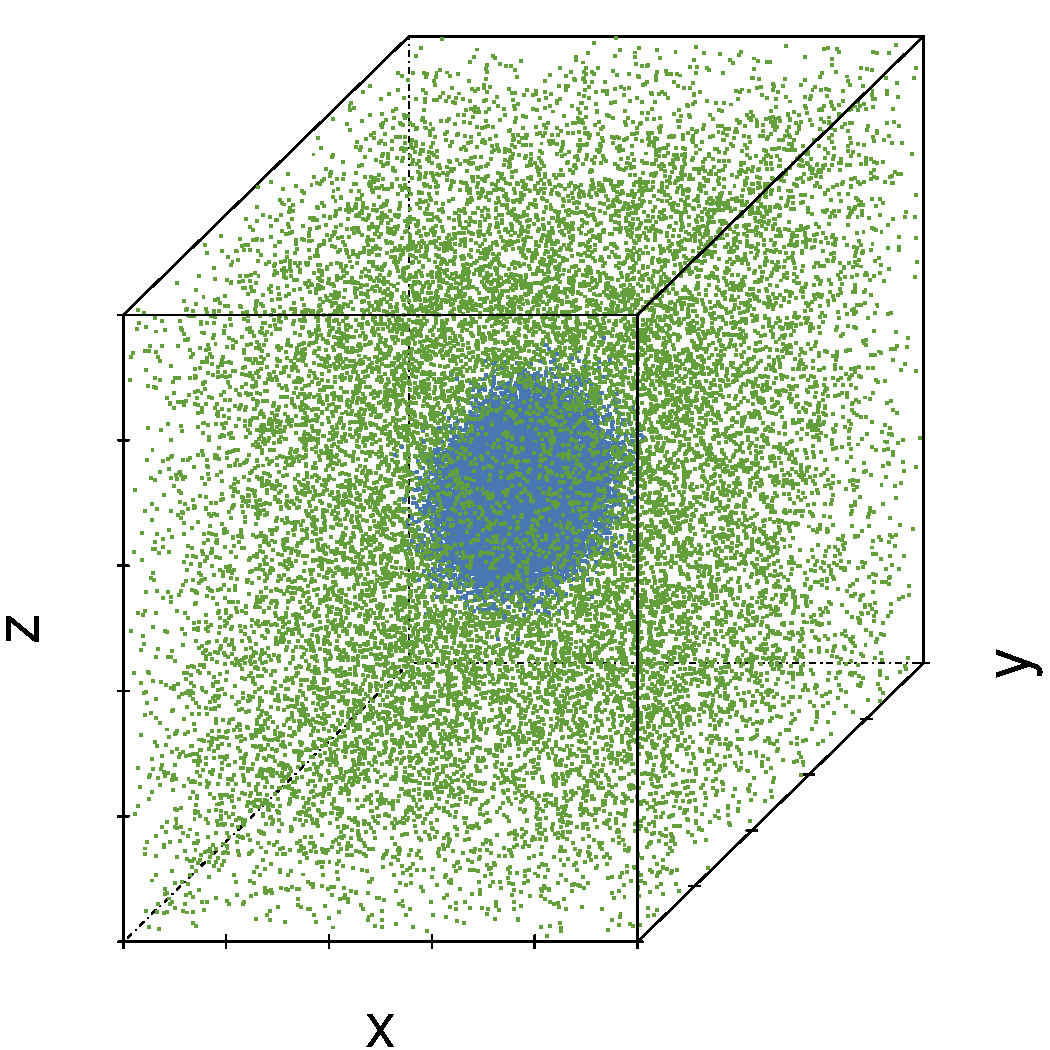
\includegraphics[width=\textwidth]{3/img/datasetplot_ferdosi_1_60000.pdf}
	\caption{Set \ferdosiOne}
	\label{fig:3:simulated:datasets:ferdosi1}
\end{subfigure}
\begin{subfigure}{0.23\textwidth}
	\centering
	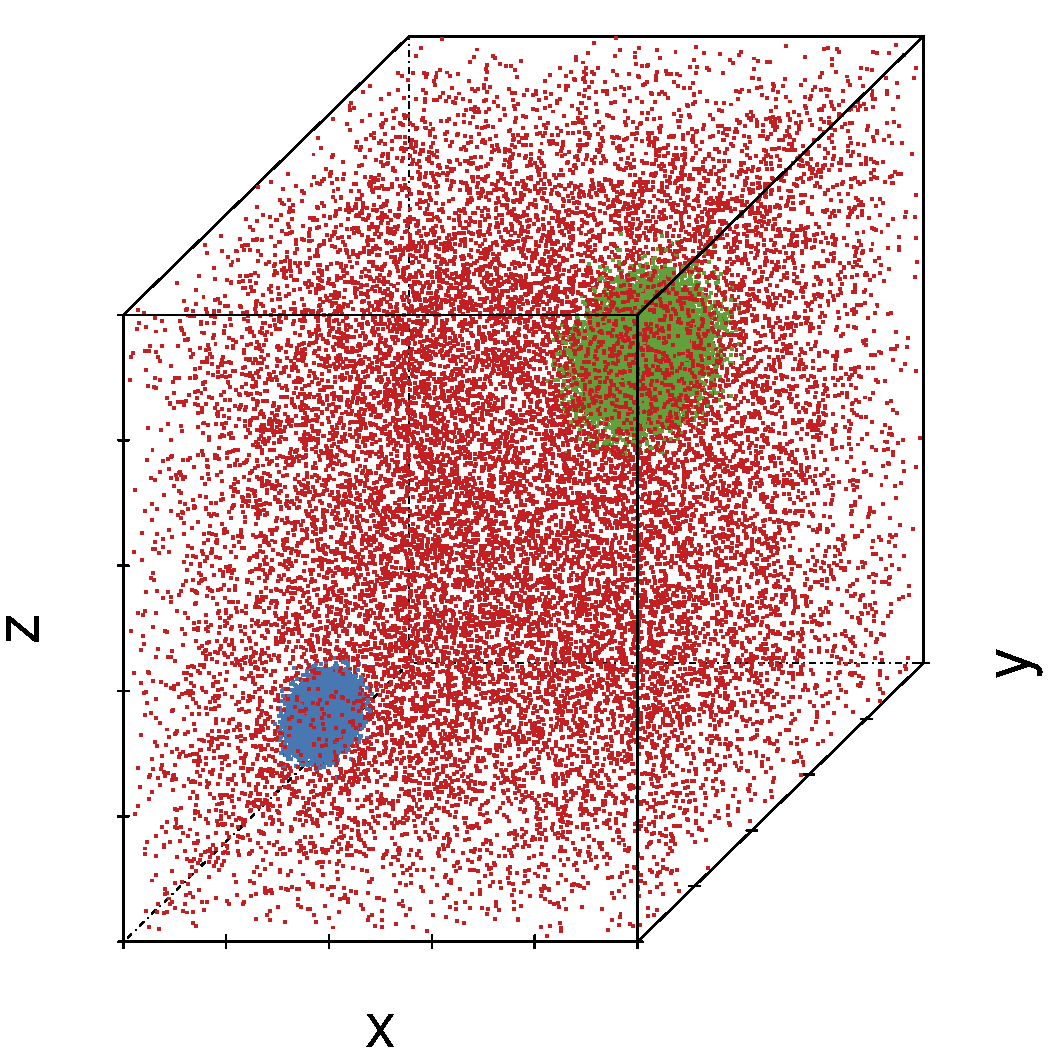
\includegraphics[width=\textwidth]{3/img/datasetplot_ferdosi_2_60000.pdf}
	\caption{Set \ferdosiTwo}
	\label{fig:3:simulated:datasets:ferdosi2}
\end{subfigure}	
\begin{subfigure}{0.23\textwidth}
	\centering
	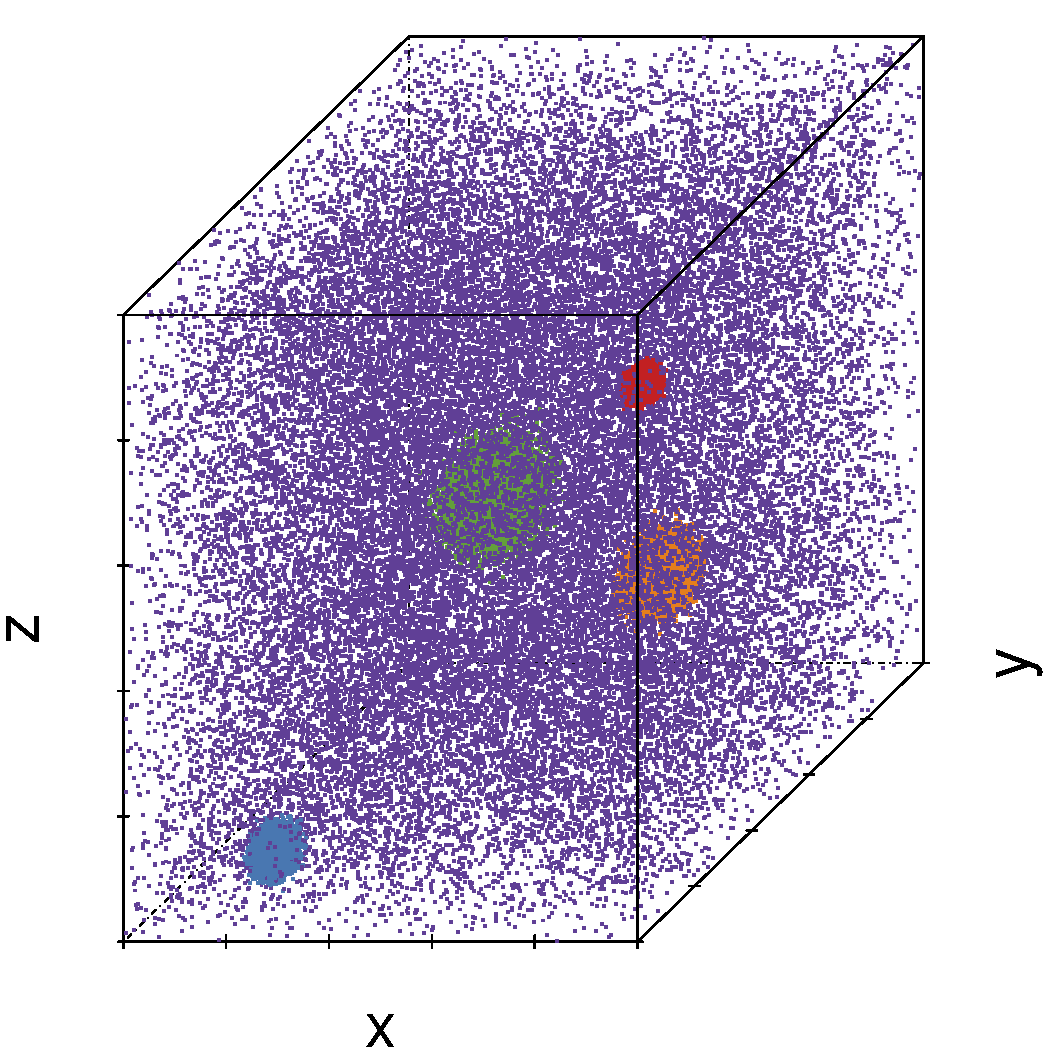
\includegraphics[width=\textwidth]{3/img/datasetplot_ferdosi_3_120000.pdf}
	\caption{Set \ferdosiThree}
	\label{fig:3:simulated:datasets:ferdosi3}
\end{subfigure}	
% Ferdosi Set 4
\begin{subfigure}{0.23\textwidth}
	\centering
	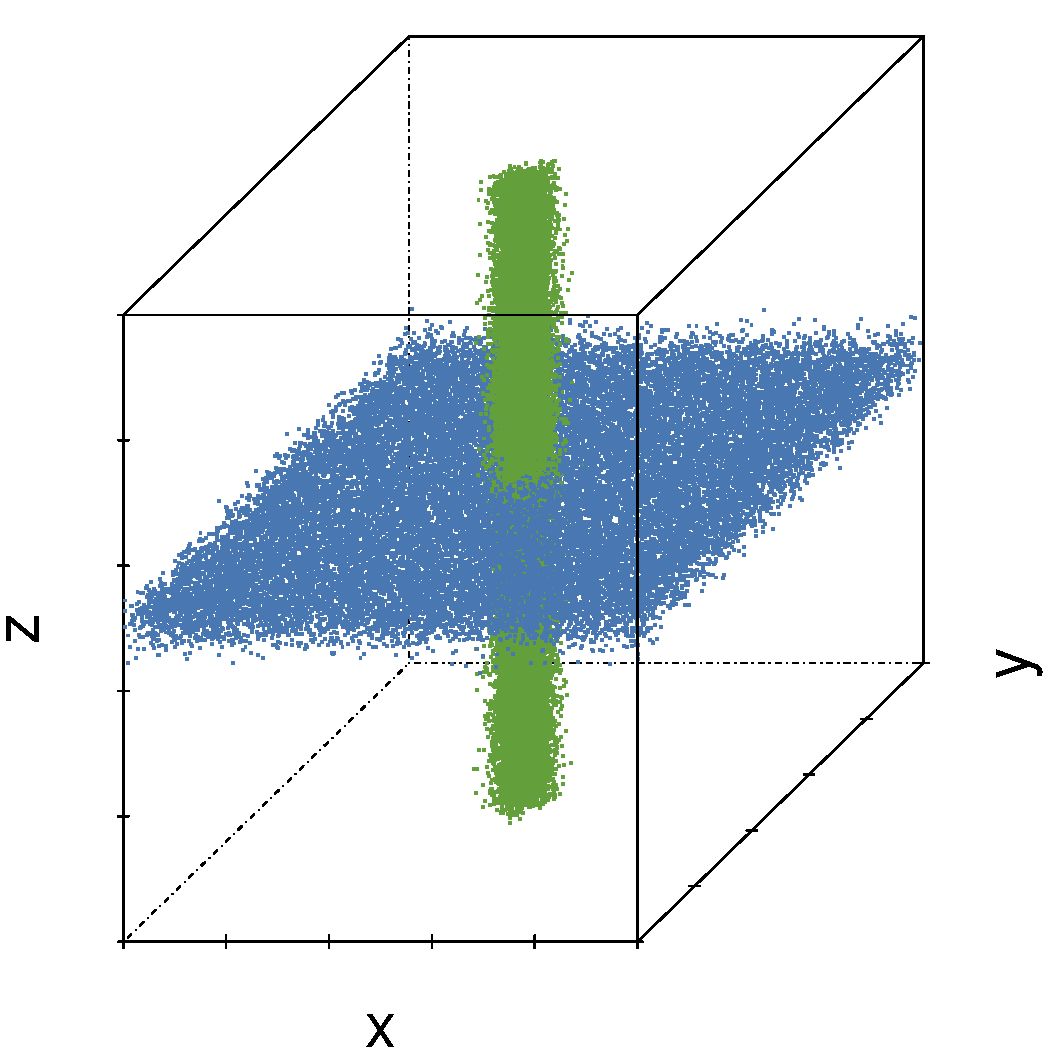
\includegraphics[width=\textwidth]{3/img/datasetplot_ferdosi_4_60000.pdf}
	\caption{Set \ferdosiFour}
	\label{fig:3:simulated:datasets:ferdosi4}
\end{subfigure}
% Baakman 1/3		
\begin{subfigure}{0.23\textwidth}
	\centering
	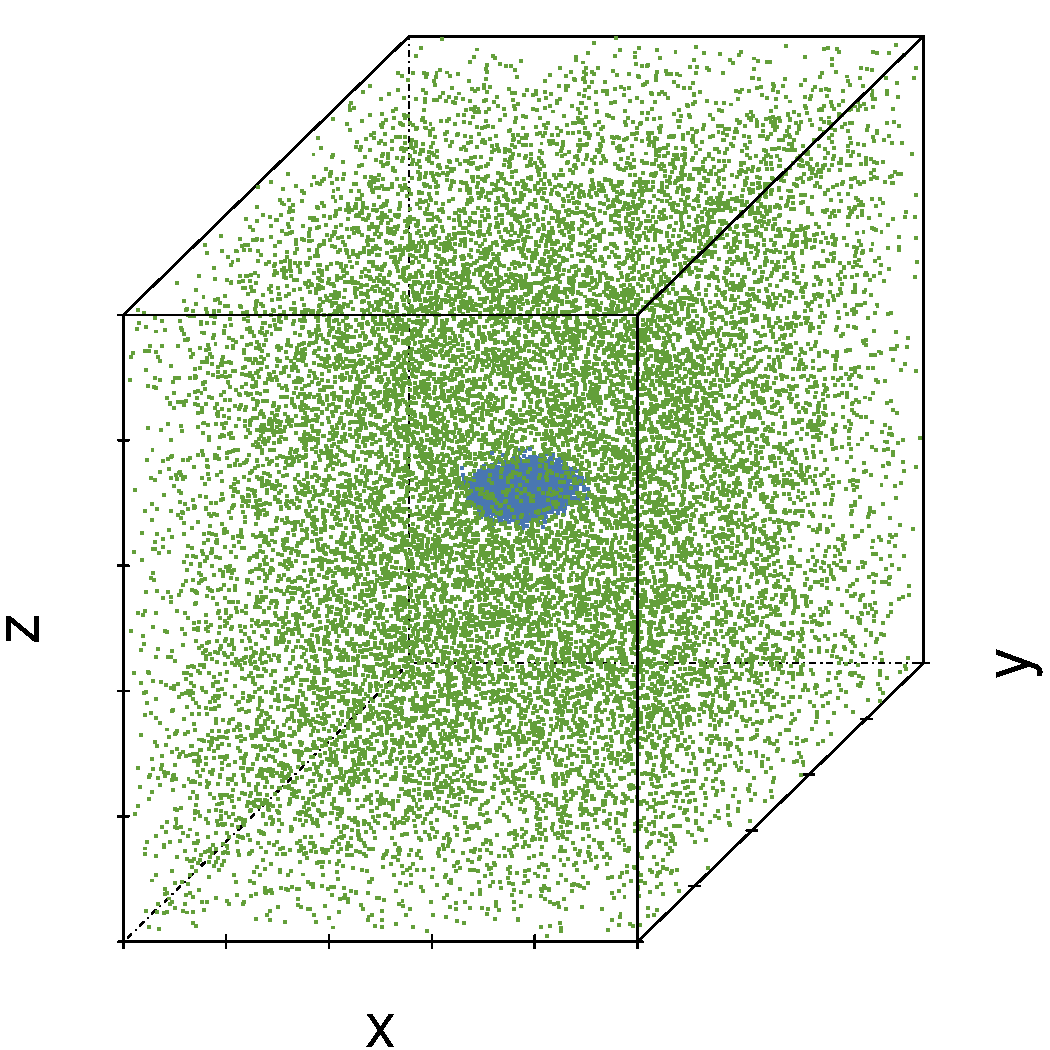
\includegraphics[width=\textwidth]{3/img/datasetplot_baakman_1_60000.pdf}
	\caption{Set 4}
	\label{fig:3:simulated:datasets:baakman1}
\end{subfigure}
\begin{subfigure}{0.23\textwidth}
	\centering
	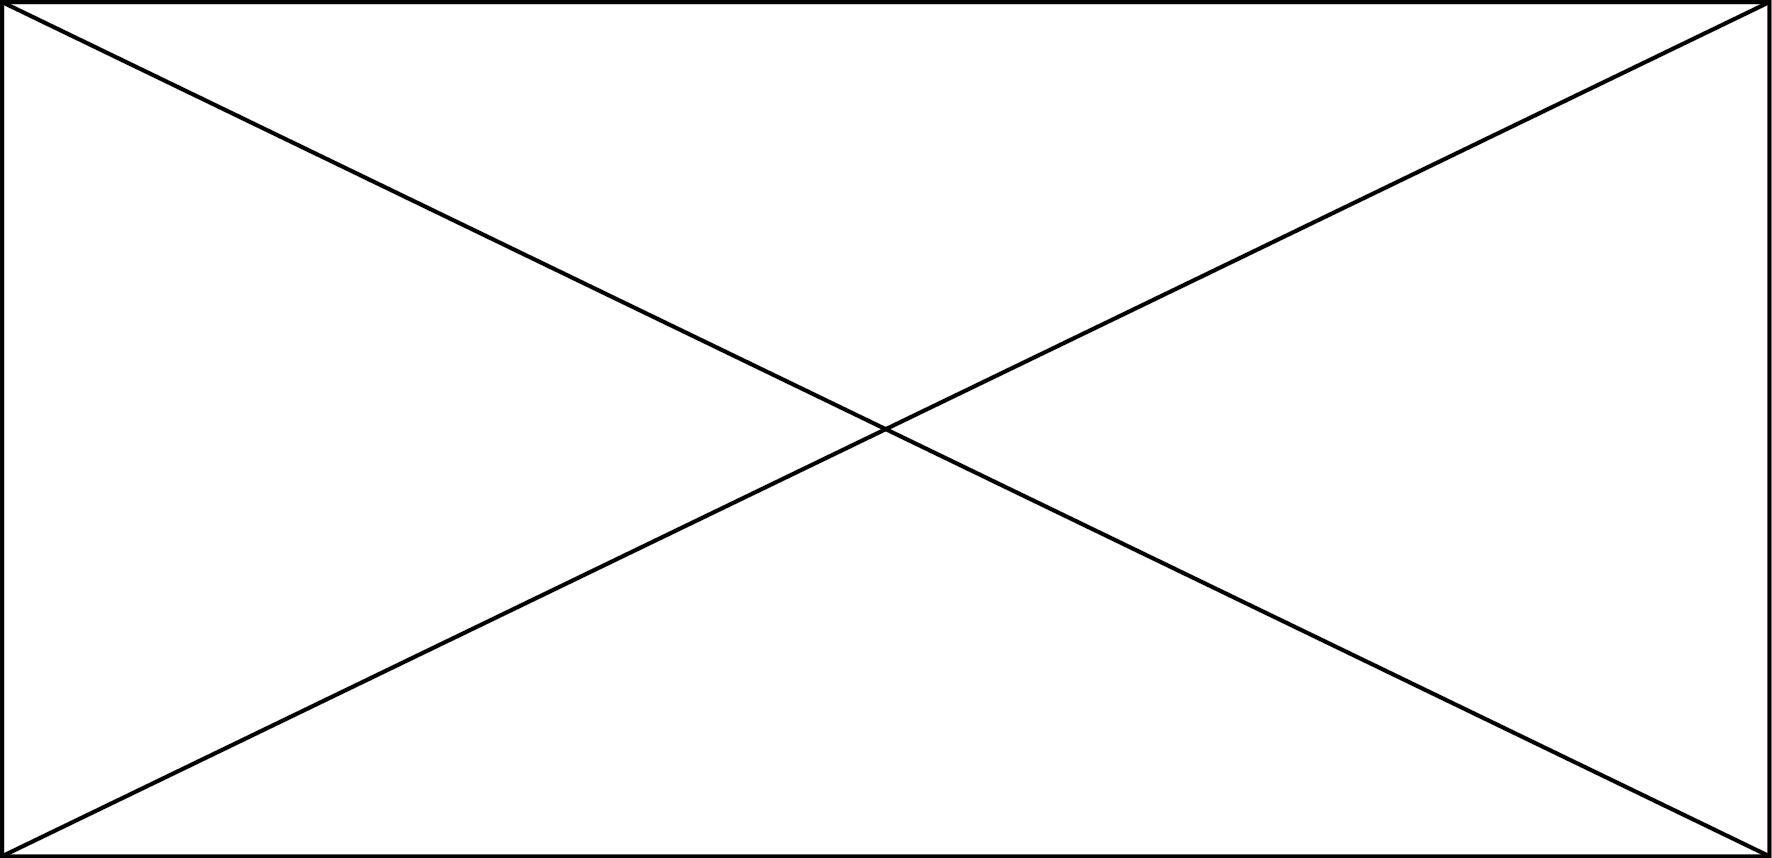
\includegraphics[width=\textwidth]{img/missingfigure.png}
	\caption{Set 5}
	\label{fig:3:simulated:datasets:baakman2}
\end{subfigure}	
\begin{subfigure}{0.23\textwidth}
	\centering
	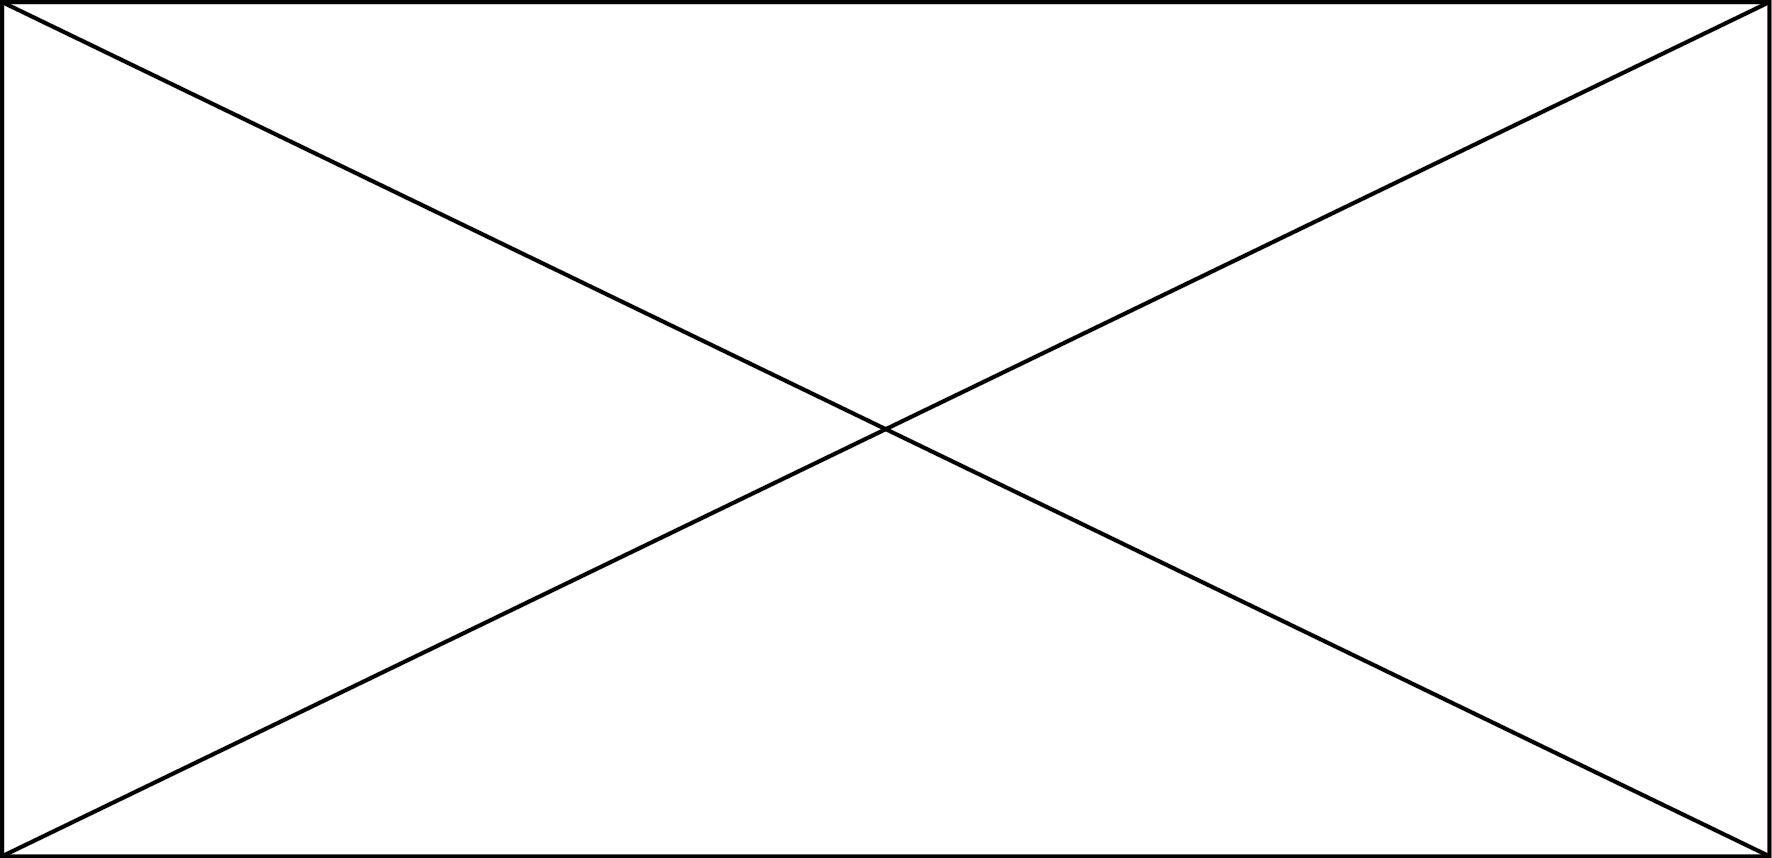
\includegraphics[width=\textwidth]{img/missingfigure.png}
	\caption{Set 6}
	\label{fig:3:simulated:datasets:baakman3}
\end{subfigure}			
% Ferdosi 5
\begin{subfigure}{0.23\textwidth}
	\centering
	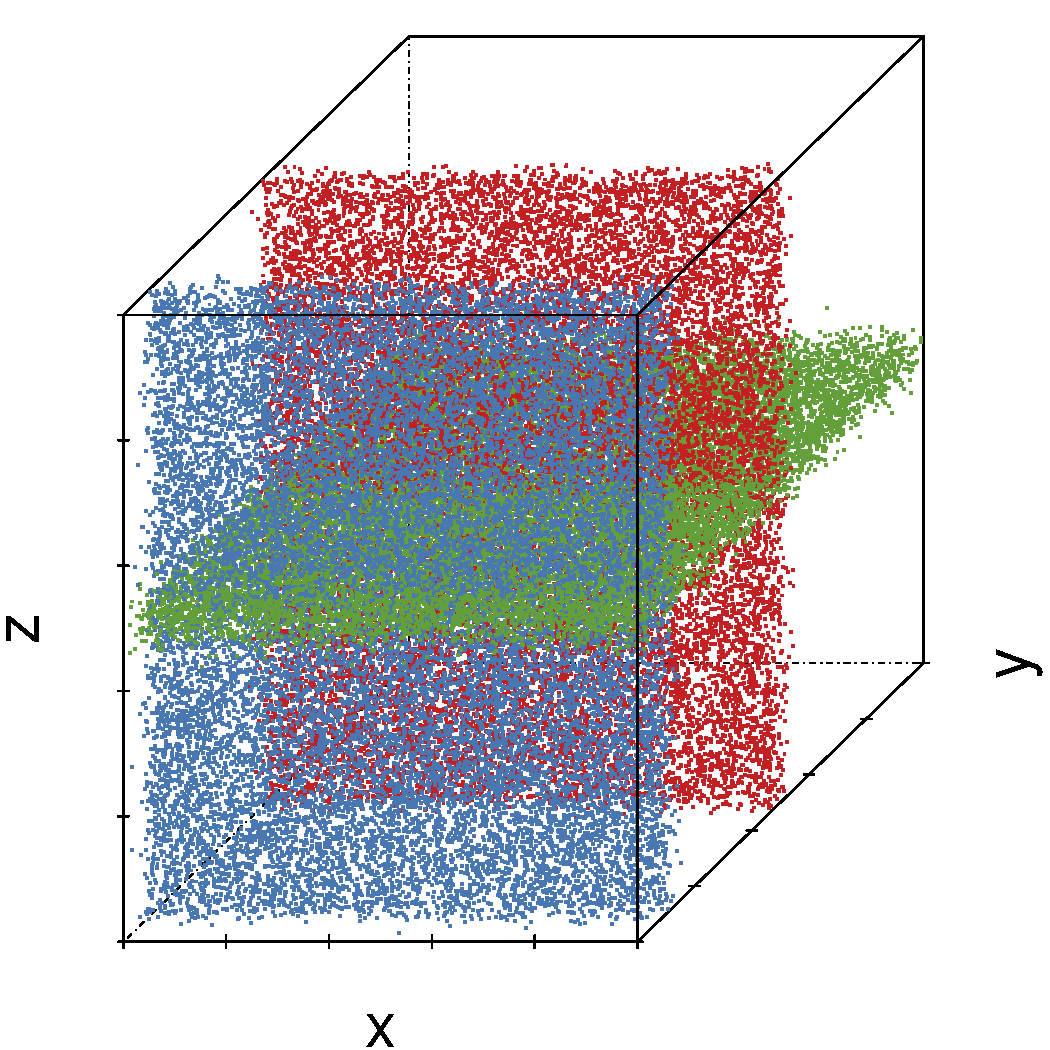
\includegraphics[width=\textwidth]{3/img/datasetplot_ferdosi_5_60000.pdf}
	\caption{Set 8}
	\label{fig:3:simulated:datasets:ferdosi5}
\end{subfigure}	